\documentclass[UTF8,12pt,a4paper,fontset=none]{ctexart}
\setCJKmainfont[AutoFakeSlant=0.2]{Noto Serif CJK SC}
\setCJKsansfont{Noto Sans CJK SC}
\setCJKmonofont{Noto Sans Mono CJK SC}
\usepackage{amsmath,amssymb,mathtools}
\usepackage{booktabs,array,tabularx,longtable,multirow}
\usepackage{geometry,graphicx,xcolor,enumitem,caption,float}
\usepackage[hidelinks]{hyperref}
\geometry{left=2.2cm,right=2.2cm,top=2.1cm,bottom=2.1cm}
\definecolor{navy}{HTML}{12324A}
\definecolor{teal}{HTML}{287C8E}
\definecolor{gold}{HTML}{D19A39}
\definecolor{brick}{HTML}{B85C38}
\definecolor{audit}{HTML}{FFF1EE}
\definecolor{auditline}{HTML}{B85C38}
\definecolor{softblue}{HTML}{EAF3F6}
\hypersetup{colorlinks=true,linkcolor=navy,urlcolor=teal}
\captionsetup{font=small,labelfont=bf}
\setlist{itemsep=2pt,topsep=3pt}
\newcommand{\keywords}[1]{\par\noindent\textbf{关键词：}#1}
\newcommand{\auditbox}[2]{\begin{center}\fcolorbox{auditline}{audit}{\begin{minipage}{0.92\linewidth}\textbf{#1}\quad #2\end{minipage}}\end{center}}
\newcommand{\status}{\textcolor{brick}{\texttt{FEASIBLE}}}
\title{\textcolor{navy}{第二题：伴随保障编组与工作负荷均衡}\\[-2pt]\large 队内阶段性建模与复核简报}
\author{数学建模小组}
\date{2026年11月21日}
\begin{document}
\maketitle
\begin{center}
\fcolorbox{navy}{softblue}{\begin{minipage}{0.92\linewidth}
\textbf{本稿定位。} 本报告把问题2的受限候选、排程复核和后续建模任务整理成可讨论版本。三个情景均找到可行排程，但求解状态均为 \status{}；它们不构成资源最少或负荷极差全局最小的证明。数值来自\texttt{q2\_fair\_b16.json}、\texttt{q2\_fair\_b24.json}和\texttt{q2\_fair\_b30.json}，并通过\texttt{验证问题2候选.py}独立复核。
\end{minipage}}
\end{center}
\begin{abstract}
第二题要求在 $120$ 分钟内完成 $32$ 架 A 型机与 $16$、$24$ 或 $30$ 架 B 型机的首次保障，并由 N 地勤派出人员和车辆随队进驻、加入 M 地勤的保障序列。本文沿队友文档的“题意分析—模型假设—资源核算—求解结果—审计提示”结构，给出当前可复核的流程、资源配置和组级负荷比较。当前候选使用 M/N 联合资源池、第一技能和跨机型 $0.9$ 熟练度，航材按全部飞机的保守假设处理，电源/空调按逐机占车处理。Z3/Z4 的车辆口径已明确为每辆车及其操作员可在同一时段服务最多 $10$ 架飞机；完整批次模型和第二、第三技能仍需重算。
\keywords{伴随保障；模块化编组；资源受限调度；工作强度均衡；可复核候选}
\end{abstract}
\section{问题分析}
本问的任务不是让 N 地勤独立完成 B 机保障，而是让 N 方携带部分人车随同 B 机转场，进驻后与 M 方资源合并调配。三个机队组合为
\[
 (A,B)\in\{(32,16),(32,24),(32,30)\},\qquad T=120\ \text{min}.
\]
排程的关键在于同时处理工序先后、车辆容量、人员技能和 M/N 来源。我们沿队友文档的写法，先把流程图转为有向工序网，再把人员和车辆写入资源容量约束，最后以 CP-SAT 生成逐机工序记录。
\begin{figure}[H]
\centering
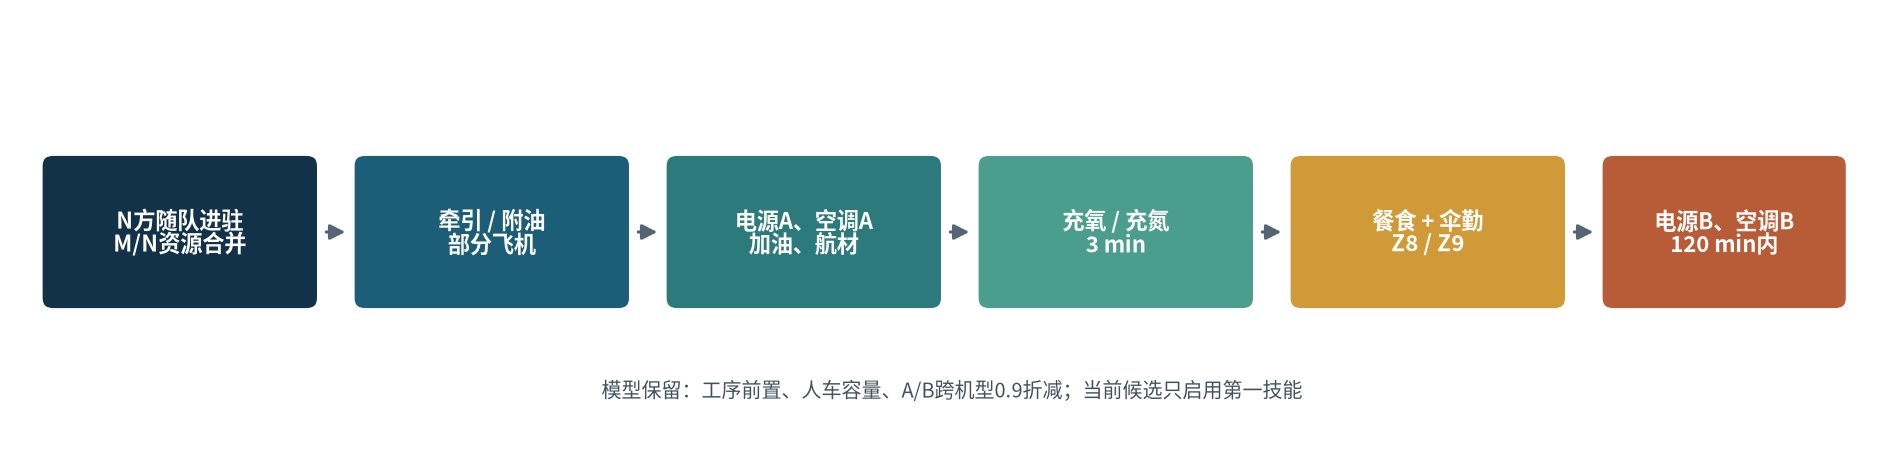
\includegraphics[width=0.98\linewidth]{figures/flow.png}
\caption{问题2候选采用的首次保障工序链与 M/N 资源合并过程。}
\label{fig:q2-flow}
\end{figure}
\auditbox{审计提示 01}{队友文档指出，Z3/Z4 的“每 $10$ 架配 $1$ 辆”不能直接理解为一辆车只能顺序服务 $10$ 架。当前统一采用并发口径：每辆 Z3 或 Z4 及其一名操作员可在同一时间段服务至多 $10$ 架；因此车辆数量下界为 $\lceil n/10\rceil$，批内任务仍须按车辆和操作员逐时核对。}
\section{模型假设与符号}
\subsection{流程与资源}
对飞机 $i$ 和工序 $o$ 设开始、结束时刻为 $s_{i,o}$ 与 $c_{i,o}$，工序时长为 $p_{i,o}$。图1的主链写为
\[
 c_{i,o}=s_{i,o}+p_{i,o},\qquad s_{i,o'}\geq c_{i,o}\quad ((o,o')\in E),
\]
其中 $E$ 包含：牵引后方可开始电源 A、空调 A、加油和附油；加油、电源 A、空调 A 完成后方可充氧、充氮；气体作业完成后方可餐食；餐食完成后方可进行电源 B、空调 B。航材和伞勤按候选的批次记录插入餐食前。
人员按来源 $h\in\{M,N\}$ 和专业组 $g$ 记录，车辆按车型 $v$ 记录。当前候选保留附录3的跨机型熟练度 $0.9$，即由另一机型来源承担任务时用时放大为 $p/0.9$。第二、第三技能的 $0.8/0.4$ 折减尚未放入本轮候选。
\begin{table}[H]
\centering\small
\caption{问题2候选中的主要资源与功能包}
\label{tab:q2-resource}
\begin{tabularx}{\linewidth}{>{\bfseries}l l X l}
\toprule
功能 & 车辆 & 人员组 & 当前处理方式\\
\midrule
牵引 & Z1 & M5 & 按机队总量的10\%向上取整，固定对象\\
加油 & Z2 & M6 & A/B工时分别15/30分钟，车辆逐机占用\\
充氧、充氮 & Z3、Z4 & M8 & 车辆数按$\lceil n/10\rceil$核对，完整批次模型待重算\\
电源、空调 & Z5、Z6 & M7 & 当前候选按逐机占车，尚未使用每车最多2架的配对能力\\
餐食 & Z8 & M1 & A/B工时分别8/25分钟，餐食需在气体作业后\\
航材、伞勤 & Z9 & M3/M4 & 以M方固定批次承担，属于保守口径\\
\bottomrule
\end{tabularx}
\end{table}
\subsection{工作强度指标}
对有 N 方派出人员的专业组 $g$，令 $L_g$ 为该组实际人·分钟工作量，$y_g$ 为 N 方派出人数，组平均利用率定义为
\[
 r_g=\frac{L_g}{120y_g},\qquad y_g>0.
\]
候选的公平指标为有任务组的利用率极差
\[
 R=\max_{g:y_g>0}r_g-\min_{g:y_g>0}r_g.
\]
公平候选固定资源向量后重新排程并压低 $R$，所以它回答的是“给定派遣规模后如何排得更均衡”，不等价于联合最小化人数、车辆和极差。
\section{候选求解与复核链}
当前候选通过三个步骤生成：
\begin{enumerate}
  \item 读取已规范化的题面数据和 M/N 资源库存，按三种 B 机数量展开飞机列表；
  \item 以 CP-SAT 建立每架飞机的工序区间、M/N 来源选择、人员累计容量和车辆累计容量，并固定牵引/附油对象及航材批次；
  \item 用独立脚本重算工序时长、前置关系、120分钟时限、峰值资源、车辆库存及 Z3/Z4 数量规则。
\end{enumerate}
\begin{figure}[H]
\centering
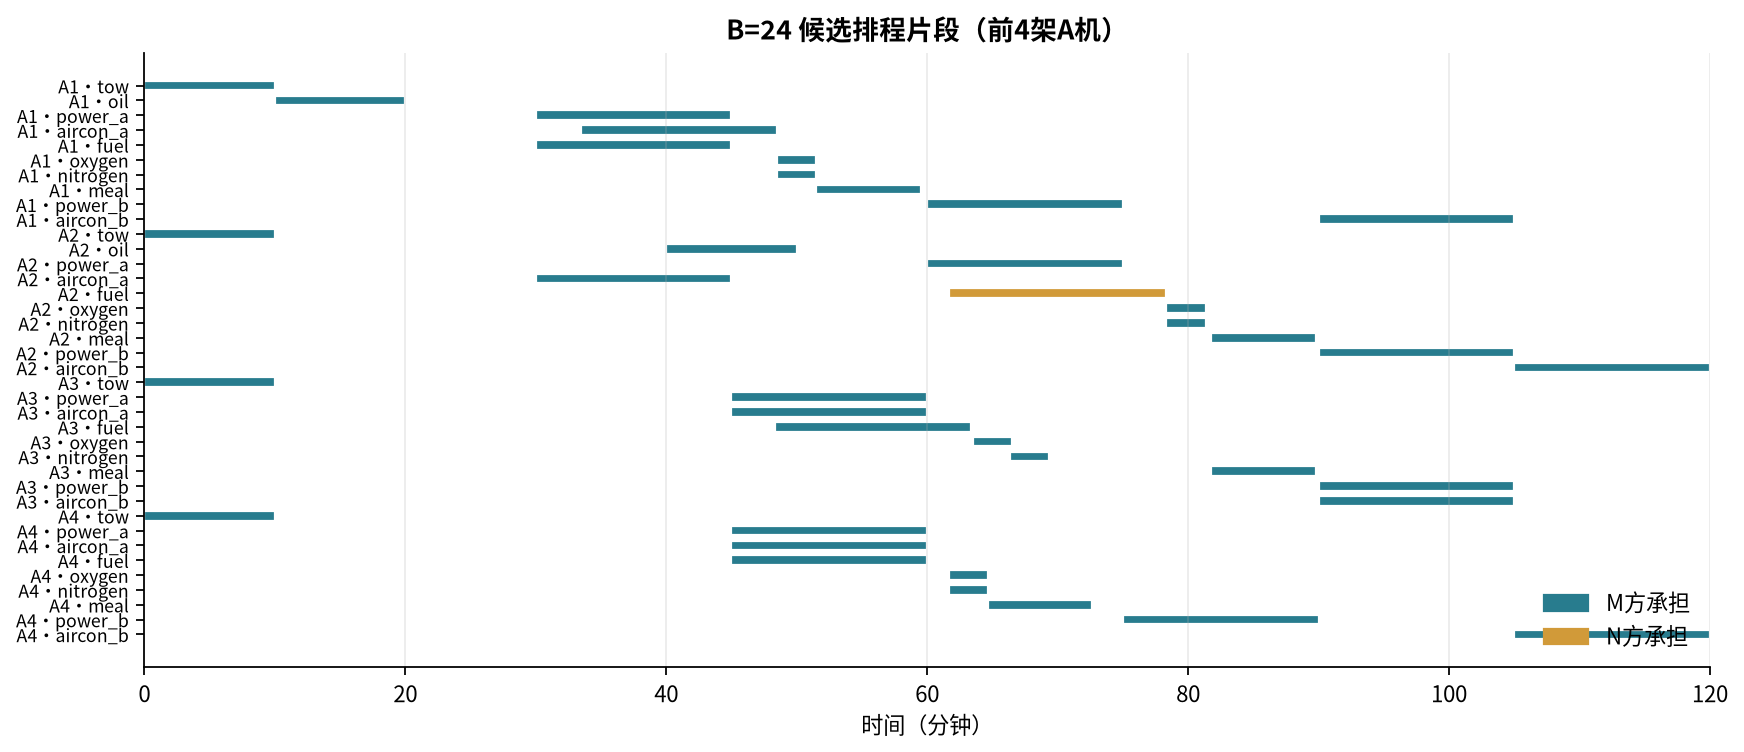
\includegraphics[width=0.92\linewidth]{figures/gantt_b24.png}
\caption{$32$A+$24$B 候选排程片段：展示前4架 A 机的工序和 M/N 来源；完整 JSON 包含全部飞机记录。}
\label{fig:q2-gantt}
\end{figure}
三个候选均通过独立复核，且复核输出中没有资源峰值超限或工序前置错误。复核覆盖当前代码实现的约束，不覆盖尚未实现的第二、第三技能替代、完整模块绑定和全局最优性。
\section{三种机队组合的资源结果}
表\ref{tab:q2-dispatch}给出 N 方派遣资源。人员和车辆数均为 JSON 中的派出量，状态保留为 \status{}。Z3 只列 N 方新增量；总量应与 M 方库存相加后再按 $\lceil (32+B)/10\rceil$ 规则核对。
\begin{table}[H]
\centering\small
\caption{三种机队组合的 N 方派遣候选}
\label{tab:q2-dispatch}
\begin{tabularx}{\linewidth}{c X X c}
\toprule
B机数 & 派出人员（专业组：人数） & 派出车辆（车型：数量） & 状态\\
\midrule
16 & M1:2，M6:1，M7:7（合计10人） & Z2:2，Z3:1，Z8:3，Z9:1（合计7辆） & \status{}\\
24 & M1:4，M6:4，M7:12（合计20人） & Z2:7，Z3:2，Z5:1，Z6:1，Z8:7，Z9:1（合计19辆） & \status{}\\
30 & M1:10，M6:3，M7:16（合计29人） & Z2:11，Z3:3，Z5:3，Z6:3，Z8:11，Z9:1（合计32辆） & \status{}\\
\bottomrule
\end{tabularx}
\end{table}
\begin{figure}[H]
\centering
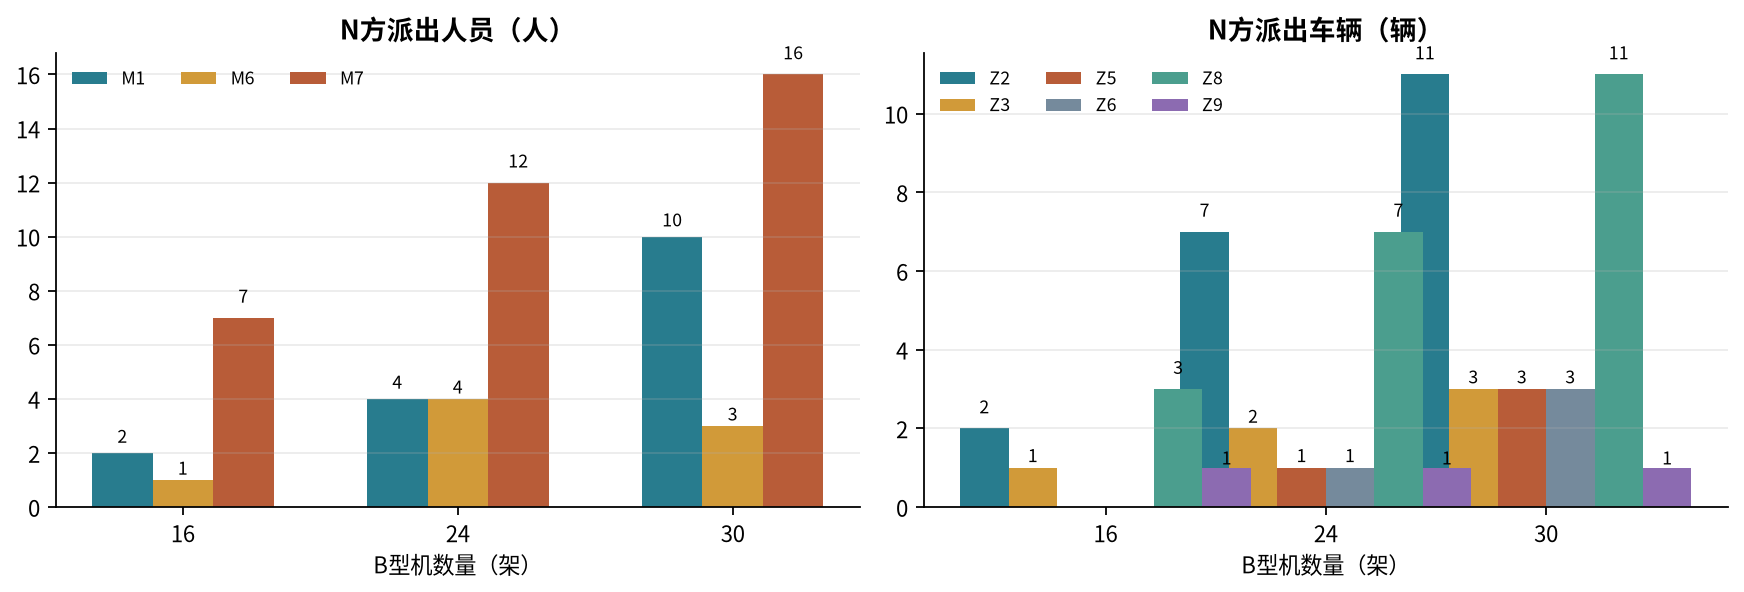
\includegraphics[width=0.96\linewidth]{figures/dispatch.png}
\caption{N 方派出人员与车辆随 B 型机数量变化。图中只显示有派出量的主要专业组和车型。}
\label{fig:q2-dispatch}
\end{figure}
车辆必要下界的当前核对为：总机队为48、56、62架时，Z3/Z4各至少需5、6、7辆；M方库存已覆盖Z4，Z3分别需N方补1、2、3辆。这个下界只来自车辆数量规则和必要容量，不能单独证明完整排程可行，更不能推出 N 方总车辆数的全局最优。
\section{工作负荷均衡结果}
\begin{table}[H]
\centering\small
\caption{固定派遣配置下的 N 方组平均利用率}
\label{tab:q2-fair}
\begin{tabular}{c c c c c}
\toprule
B机数 & M1餐食 & M6加油 & M7电源空调 & 极差\\
\midrule
16 & 57.87\% & 63.89\% & 69.64\% & 11.77个百分点\\
24 & 57.18\% & 58.33\% & 72.92\% & 15.74个百分点\\
30 & 55.00\% & 55.56\% & 75.09\% & 20.09个百分点\\
\bottomrule
\end{tabular}
\end{table}
利用率由对应 JSON 的人·分钟工作量除以 $120y_g$ 得到。例如 $32$A+$16$B 情景中，M1、M6、M7 的工作量分别为 $138.8889$、$76.6667$ 和 $585.0000$ 人·分钟，对应派出人数为2、1、7，故利用率为57.87\%、63.89\%、69.64\%。三个情景的公平求解均为 \status{}，极差是当前固定配置下的候选值，不是已证明的最小值。
\begin{figure}[H]
\centering
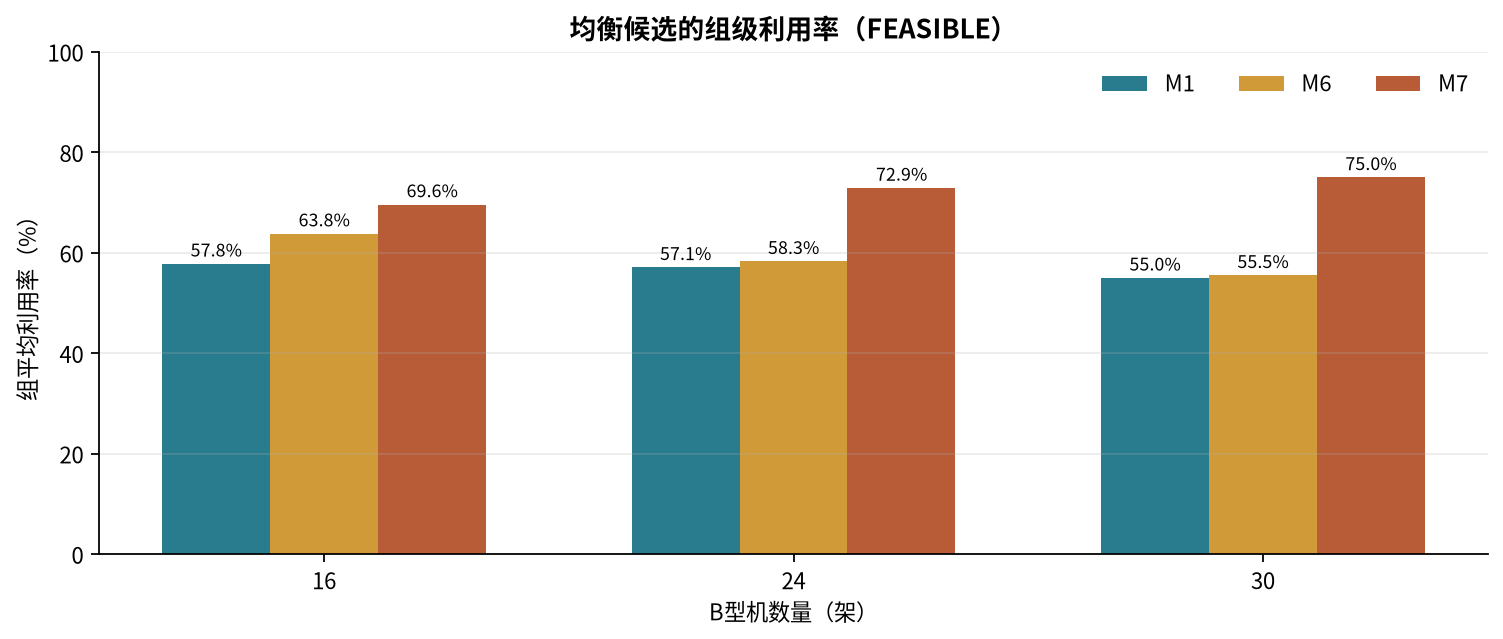
\includegraphics[width=0.88\linewidth]{figures/utilization.png}
\caption{三种机队组合的组级利用率。M7 随 B 机数量增加而成为主要负荷组。}
\label{fig:q2-util}
\end{figure}
\auditbox{审计提示 02}{组平均利用率不能替代个人负荷审计。当前个人分工采用贪心分配，尚未证明每名人员的最大工作量最小；若启用跨技能补位，还需同时检查补位人员原岗位是否被覆盖。}
\section{结果边界与下一步}
当前结果可用于队内讨论的结论有三点：
\begin{enumerate}
  \item 在当前受限模型和固定派遣配置下，三种机队组合均得到120分钟内的可行候选，且独立复核通过；
  \item 固定配置后重新排程可以把三组平均利用率极差压到11.77、15.74和20.09个百分点；
  \item 现有候选显示 M7 电源空调组在三种情景中负荷最高，下一轮应优先把第二技能和每车同时服务2架的配对约束加入同一个模型。
\end{enumerate}
下列事项完成前，不把当前表格写成正式最优配置：
\begin{itemize}
  \item 把 Z3/Z4 明确写成不超过10架的并发批次，每批绑定1辆车和1名操作员，并同时检查 M8 人员；
  \item 把电源/空调的“一车一人、同时最多2架”配对能力写入区间模型，比较逐机占车和配对占车两种口径；
  \item 实现第二、第三技能的 $0.8/0.4$ 折减，联合优化 M/N 来源、模块编组和资源非支配解；
  \item 取得官方 \texttt{C\_Solution1.xlsx} 或按附录9重建并逐字段填表，保留候选 JSON、复核日志和结果哈希。
\end{itemize}
\section{复现清单}
\begin{table}[H]
\centering\small
\caption{本报告使用的主要文件}
\begin{tabularx}{\linewidth}{l X}
\toprule
用途 & 文件\\
\midrule
题面与规范化输入 & \texttt{data/新2026C.docx}；\texttt{results/q23\_normalized.json}\\
三组公平候选 & \texttt{results/q2\_fair\_b16.json}、\texttt{q2\_fair\_b24.json}、\texttt{q2\_fair\_b30.json}\\
独立复核 & \texttt{验证问题2候选.py}\\
车辆下界 & \texttt{results/q2\_vehicle\_lower\_bounds.csv}\\
图表生成 & \texttt{figures/generate\_q2\_figures.py}\\
\bottomrule
\end{tabularx}
\end{table}
\vfill
\begin{center}\small\textcolor{navy}{本 PDF 是队内阶段性讨论材料；所有数值都带有当前模型范围和状态标签，提交前仍需人工核对题面口径、正式模板和完整求解结果。}\end{center}
\end{document}
